\documentclass[12pt,aspectratio=43]{beamer}
\usepackage{tikz}
\usetheme{Madrid}
\setbeamertemplate{navigation symbols}{}
\title{Incremental analysis: experiments and bounds}
\subtitle{Generated interaction study}
\author{Research group}
\date{}
\year=2026\month=11\day=5
\newcommand{\fuzzlayerA}[1]{\textbf{#1}}
\newcommand{\fuzzlayerB}[1]{\fuzzlayerA{#1}}
\newcommand{\fuzzlayerC}[1]{\fuzzlayerB{#1}}
\newcommand{\fuzzterm}[1]{\fuzzlayerC{#1}}
\newcommand{\fuzzpair}[2]{\fuzzterm{#1}: #2}
\newcommand{\fuzzunit}{steps}
\let\fuzzoriginalunit\fuzzunit
\newcommand{\fuzzcoefficient}{4}
\newcommand{\fuzzscale}[2][\fuzzcoefficient]{#1\,#2}
\definecolor{fuzzpaint}{RGB}{255,0,255}
\definecolor{fuzzsecond}{RGB}{18,137,67}
\tikzset{fuzzvertex/.style={draw,rounded corners=1pt,fill=blue!10,inner sep=1pt,minimum width=.35cm,minimum height=.25cm}}
\begin{document}\begin{frame}[t,shrink=5]{Block column boundary}
Before.\par\begin{alertblock}{Geometric uncertainty}
\begin{columns}[onlytextwidth,t]
\begin{column}{0.38\textwidth}
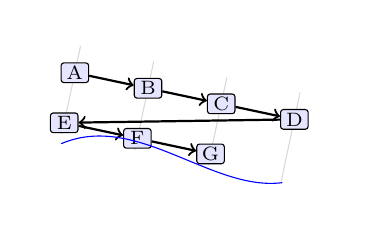
\begin{tikzpicture}[font=\scriptsize]
\begin{scope}[scale=1,rotate=-12]
\clip (-.4,-1) rectangle (3.350,.5);
\foreach \x in {0,1,2,3} {\draw[gray!30] (\x*0.950,-.8)--(\x*0.950,.35);}
\node[fuzzvertex] (g3n0) at (0.000,0) {A};
\node[fuzzvertex] (g3n1) at (0.950,0) {B};
\node[fuzzvertex] (g3n2) at (1.900,0) {C};
\node[fuzzvertex] (g3n3) at (2.850,0) {D};
\node[fuzzvertex] (g3n4) at (0.000,-0.65) {E};
\node[fuzzvertex] (g3n5) at (0.950,-0.65) {F};
\node[fuzzvertex] (g3n6) at (1.900,-0.65) {G};
\begin{scope}[xshift=.5pt,yshift=-.5pt]
\draw<1->[->,thick] (g3n0) -- (g3n1);
\draw<1->[->,thick] (g3n1) -- (g3n2);
\draw<1->[->,thick] (g3n2) -- (g3n3);
\draw<1->[->,thick] (g3n3) -- (g3n4);
\draw<1->[->,thick] (g3n4) -- (g3n5);
\draw<1->[->,thick] (g3n5) -- (g3n6);
\draw[blue] (0,-.9) .. controls (0.855,-.3) and (1.995,-1.1) .. (2.850,-.8);
\end{scope}
\end{scope}
\end{tikzpicture}
\end{column}
\begin{column}{0.58\textwidth}
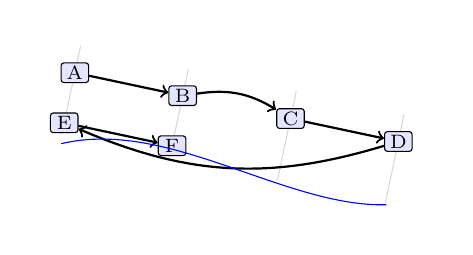
\begin{tikzpicture}[font=\scriptsize]
\begin{scope}[scale=1,rotate=-12]
\clip (-.4,-1) rectangle (4.700,.5);
\foreach \x in {0,1,2,3} {\draw[gray!30] (\x*1.400,-.8)--(\x*1.400,.35);}
\node[fuzzvertex] (g4n0) at (0.000,0) {A};
\node[fuzzvertex] (g4n1) at (1.400,0) {B};
\node[fuzzvertex] (g4n2) at (2.800,0) {C};
\node[fuzzvertex] (g4n3) at (4.200,0) {D};
\node[fuzzvertex] (g4n4) at (0.000,-0.65) {E};
\node[fuzzvertex] (g4n5) at (1.400,-0.65) {F};
\begin{scope}[xshift=.5pt,yshift=-.5pt]
\draw<2->[->,thick] (g4n0) -- (g4n1);
\draw<2->[->,thick] (g4n1) to[bend left=20] (g4n2);
\draw<2->[->,thick] (g4n2) -- (g4n3);
\draw<2->[->,thick] (g4n3) to[bend left=20] (g4n4);
\draw<2->[->,thick] (g4n4) -- (g4n5);
\draw[blue] (0,-.9) .. controls (1.260,-.3) and (2.940,-1.1) .. (4.200,-.8);
\end{scope}
\end{scope}
\end{tikzpicture}
\end{column}
\end{columns}
\par
\begin{enumerate}
\item \begin{center}
\textrm{A local update} can change the measurements used by several neighboring components.  The estimate is $\sum_{i=1}^{n}x_i$.
\end{center}
\item \begin{flushleft}
\textrm{The next pass} must preserve the boundary conditions while revisiting dependent values. A narrow column can change line breaking even when the underlying expression is unchanged. The estimate is $\frac{a+b}{1+c}$.
\end{flushleft}
\end{enumerate}
\end{alertblock}\par Witness.\only<4>{}\end{frame}\end{document}
